% Copyright 2007 by Till Tantau
%
% This file may be distributed and/or modified
%
% 1. under the LaTeX Project Public License and/or
% 2. under the GNU Public License.
%
% See the file doc/licenses/LICENSE for more details.


\documentclass{beamer}

% Setup appearance:

\usetheme{PaloAlto}
\usefonttheme{structurebold}
%\usecolortheme{crane}
\definecolor{mygold}{RGB}{255,204,0}
\definecolor{chocolate}{RGB}{97,51,24}
\definecolor{mygreen}{RGB}{173,214,50}
\setbeamercolor{structure}{bg=chocolate, fg=white}
\setbeamercolor{palette primary}{use=structure,fg=mygold,bg=chocolate}
\setbeamercolor{sidebar}{bg=chocolate,fg=white}
\setbeamercolor{sidebar}{parent=palette primary}
\setbeamercolor{section in sidebar shaded}{fg= mygold}
\setbeamercolor{subsection in sidebar shaded}{fg= mygreen}
\setbeamercolor{item projected}{fg=white,bg=chocolate}
\setbeamercolor{block body alerted}{bg=normal text.bg!90!chocolate}
\setbeamercolor{block body}{bg=normal text.bg!90!chocolate}
\setbeamercolor{block body example}{bg=normal text.bg!90!chocolate}
\setbeamercolor{block title alerted}{use={normal text,alerted text},fg=alerted text.fg!75!normal text.fg,bg=normal text.bg!75!chocolate}
\setbeamercolor{block title}{bg=chocolate}
\setbeamercolor{block title example}{use={normal text,example text},fg=example text.fg!75!normal text.fg,bg=normal text.bg!75!chocolate}

\addtobeamertemplate{footline}
{%
   \usebeamercolor[fg]{author in sidebar}
   \vskip-1cm\hskip10pt
   %\insertpagenumber\,/\,\insertpresentationendpage\kern1em\vskip2pt%
   \insertframenumber\,/\,\inserttotalframenumber\kern1em\vskip2pt%
}


\setbeamerfont{frametitle}{size=\normalsize,series=\bfseries}
\setbeamertemplate{navigation symbols}{}

% Standard packages

\usepackage{amsmath,amsthm,amssymb,latexsym,hyperref,url,graphicx,multicol}
\usepackage{color}
\usepackage{setspace,tikz,scalefnt}
\usepackage{multirow}
\usepackage{caption}

\graphicspath{ {./Figures/} }

\logo{
\includegraphics[scale=.3]{shield5}}

% The main document
%\setbeamercovered{transparent}

\usepackage{graphicx} % Allows including images
\usepackage{caption}
\usepackage{subcaption}
\usepackage{verbatim}
\usepackage{xcolor}

%----------------------------------------------------------------------------------------
%	TITLE PAGE
%----------------------------------------------------------------------------------------

\title[Call Center Analysis]{Analysis, Visualization, and Simulation of Call Center Data} % The short title appears at the bottom of every slide, the full title is only on the title page

%* to show who is speaking
\author[Bulger \and Schmitt]{Presented by John D. Bulger\\ Graduate Student, Analytics \& Modeling
\\ \vskip0.1in Mentored by Dr. Karl Schmitt\\ Director of Data Sciences}
\institute[VERUM]{Valparaiso University}
\date{May 3, 2019}


\begin{document}

%title page frame
\begin{frame}
\titlepage
\end{frame}

%table of contents frame

\begin{frame}{Outline}
\begin{enumerate}
    \item Background
    \medskip
    \item Data
    \medskip
    \item Statistical Analysis
    \medskip
    \item Visualization
    \medskip
    \item Simulation
\end{enumerate}
\end{frame}





\section{Background}


\begin{frame}{Background}
    \centering
    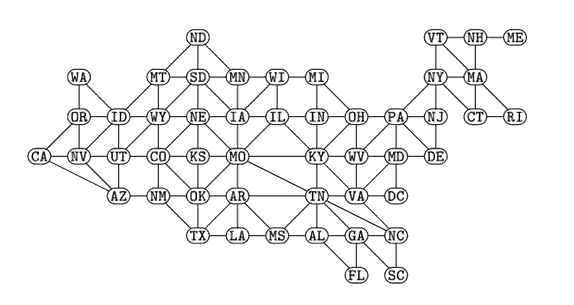
\includegraphics[scale=0.5]{contiguous-usa-graph}
    
    \tiny Retrieved from:  \url{http://mathworld.wolfram.com/images/gifs/ContiguousUSAGraph.gif}
    
\end{frame}



\begin{frame}{Project Goals}
%usebackgroundtemplate

\begin{center}
Our project aims to create a way to classify networks to facilitate research and exploration of this field.
\end{center}
\begin{enumerate}
    \item Determine characteristics of networks that make them distinct 
     \item Use machine learning to categorize miscellaneous graphs
     \item Assess the current categories and propose new ones to match our findings
  
\end{enumerate}
\end{frame}



\section{Data}

\begin{frame}{Data}
Collection or Category
\begin{itemize}
    \item Social Networks: friendships among classmates
    \item Biological Networks: food chain of an ecosystem
    \item Web Networks: links between web-pages
\end{itemize}
Features
\begin{itemize}
    \item Nodes: number of nodes
    \item Density: ratio of \# of edges to \# of possible edges
    \item Average degree: average \# of edges connected to a node
\end{itemize}
\begin{center}
    Base data-set provided by repository creators included:\\
    1241 networks with features from 20 collections
\end{center}
\end{frame}



\begin{frame}{Data Cleaning}
    \begin{itemize}
        \item Downsampled Cheminformatics (originally 6x next largest)
        \item Ended with 494 graphs and 15 collections
        \item Trained models using collections with more than 20 graphs
        \begin{itemize}
        \vspace{-\baselineskip}
            \item Reduced data to 401 graphs and 6 collections
        
        \end{itemize}

    \end{itemize}
    \begin{figure}
        \centering
        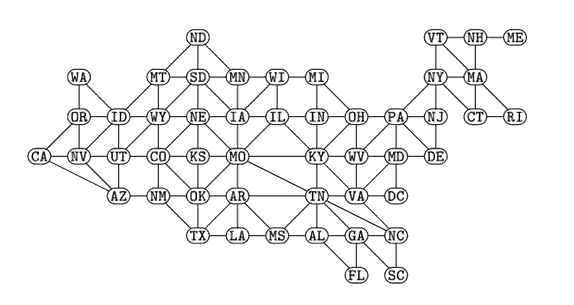
\includegraphics[scale = 0.27]{contiguous-usa-graph}
        %\caption{\scriptsize{Data After Downsampling}}
      
    \end{figure}    
    
\end{frame}
%\begin{frame}{Feature Range}
%    Add table of ranges
%    \centering
%    \includegraphics[scale=0.22]{}
%\end{frame}


\section{Statistical Analysis} 


\begin{frame}{Feature Distributions by Clusters}
    \centering
    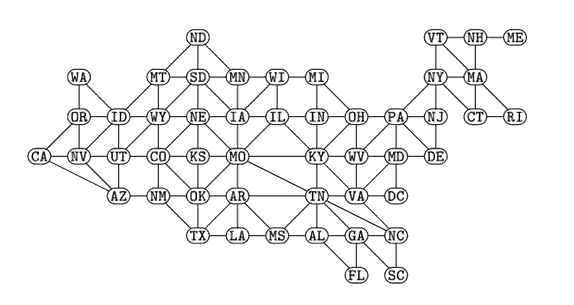
\includegraphics[scale=0.23]{contiguous-usa-graph}
\end{frame}



\begin{frame}{Supervised Machine Learning}
    \centering
    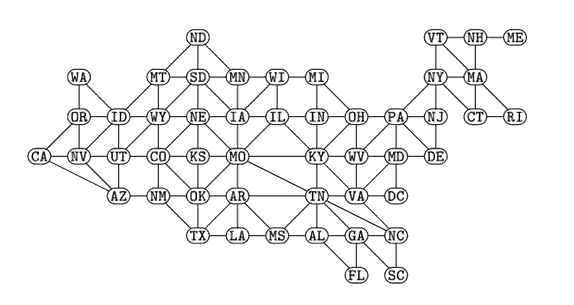
\includegraphics[scale=.5]{contiguous-usa-graph}\\
    \tiny Retrieved from:  \url{http://www.teachingdatascience.org/}
\end{frame}

 


\begin{frame}{Models}
    \begin{itemize}
        \item Decision Tree
        \item Random Forest
        \item Support Vector Classification (SVC)
        \item Linear Support Vector Classification (SVC)
        \item Logistic Regression
        \item Gaussian Na\"ive Bayes
\end{itemize}

\end{frame}



\begin{frame}{Random Forest}
    \centering
    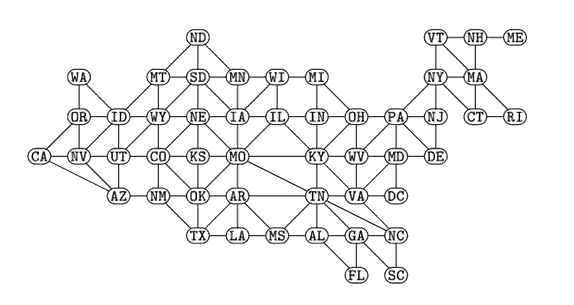
\includegraphics[scale = .3]{contiguous-usa-graph}
    
\end{frame}


\begin{frame}{Recursive Feature Elimination with Cross Validation (RFECV)}
    \begin{figure}
        \centering
        \begin{minipage}[t]{0.3\textwidth}
            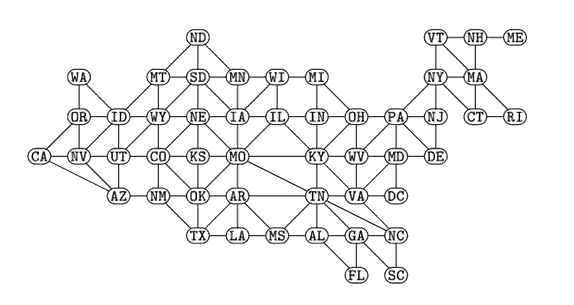
\includegraphics[scale = 0.21]{contiguous-usa-graph}
            \caption{\tiny{Decision Tree}}
            \label{fig:tree}
        \end{minipage}\hfill
        \begin{minipage}[t]{0.3\textwidth}
            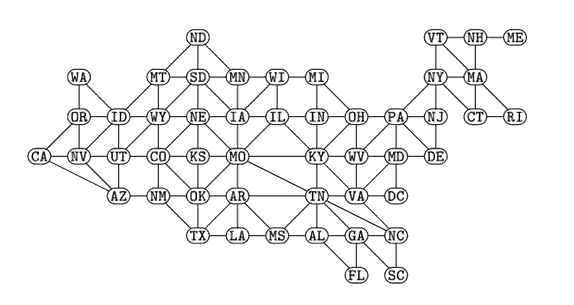
\includegraphics[scale = 0.21]{contiguous-usa-graph}
            \caption{\tiny{Random Forest}}
            \label{fig:rand_forest}
        \end{minipage}\hfill
        \begin{minipage}[t]{.3\textwidth}
            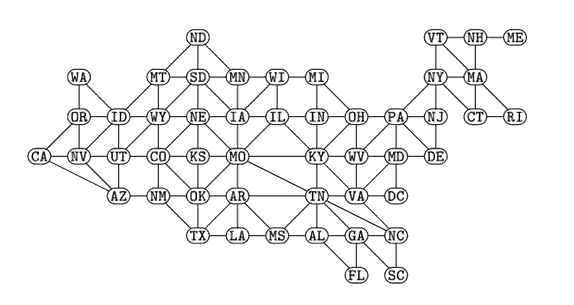
\includegraphics[scale = 0.21]{contiguous-usa-graph}
            \caption{\tiny{Linear SVC}}
            \label{fig:svc}
        \end{minipage}
    \end{figure}
    Gaussian Na\"ive Bayes
\begin{itemize}
    \item Minimum degree, maximum degree, total triangles, assortativity
\end{itemize}
    
    
\end{frame} %add comment on Gaussian NB






    
\section{Visualization}


\begin{frame}{Testing Models}

Collections of size $>$ 20

    Leave One Out cross validation 
    
    \begin{table}[]
        \centering
        \begin{tabular}{rl}
            Model & Accuracy Score \\
            Random Forest & 0.923 \\
            (reduced features) Gaussian Na\"ive Bayes &  0.920 \\
            Decision Tree & 0.914 \\
            Linear SVC & 0.803 \\
            Logistic Regression &  0.648 \\
            SVC & 0.521
        \end{tabular}

        \label{tab:my_label}
    \end{table}
    
    
    
\end{frame}


\begin{frame}{Analysis and Perspective}
\begin{itemize}
    \item \small Random Forest predictions from cross validation
    \item \small Collections are few and somewhat related
   % \item Some of these collections are related: Web Graphs, Social Networks, Facebook Networks, Retweet Networks
\end{itemize}

\center

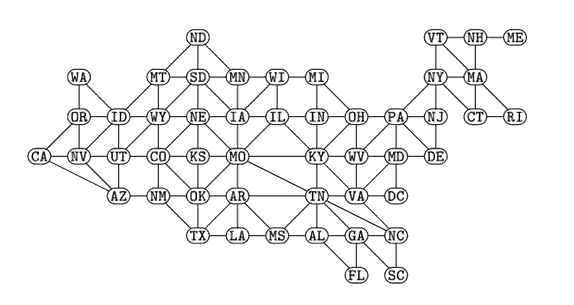
\includegraphics[scale=.6]{contiguous-usa-graph}

\medskip
\begin{table}
{\scriptsize \begin{tabular}{r r|c|c|c|c|c|c|}
  &  \multicolumn{1}{c}{} & \multicolumn{6}{c}{Predicted} \\
  & \multicolumn{1}{c}{} & \multicolumn{1}{c}{B} & \multicolumn{1}{c}{C} & \multicolumn{1}{c}{F} & \multicolumn{1}{c}{R} & \multicolumn{1}{c}{S} & \multicolumn{1}{c}{W}  \\ \cline{3-8}      
\multirow{6}{*}{\rotatebox[origin=c]{90}{Actual} }  &   Brain     &  32  &  1  &  1  &  1  &  1  & 0  \\ \cline{3-8}
  &   Chem      &  0  &  119 &  0  &  0  &  0  & 0  \\ \cline{3-8}
  &   Facebook  &  0  &  0  &  112 &  1  &  1  & 0  \\ \cline{3-8}
  &   Retweet   &  0  &  0  &  0  &  57 &  3  & 2  \\ \cline{3-8}
  &   Social    &  0  &  1  &  1  &  1  &  40  & 5  \\ \cline{3-8}
  &   Web       &  1  &  0  &  1  &  1  &  10  & 9  \\ \cline{3-8} 
\end{tabular} }
\footnotesize \caption{Confusion Matrix}
\end{table}
\end{frame}


\section{Simulation}

\begin{frame}{Motivation}
\begin{center}
Our project aims to create a way to classify networks to facilitate research and exploration of this field.
\end{center}

    \begin{itemize}
        \item Knowing the category of a graph can lead to finding established ways of working with that type of graph
        \item It can also lead to increased interdisciplinary communication
    \end{itemize}
    
\end{frame}


\begin{frame}{Mislabeled Networks}
\begin{center}
Which graph is from the Retweet Networks Collection?
\end{center}

    \begin{figure}
        \centering
        \begin{minipage}[t]{0.48\textwidth}
            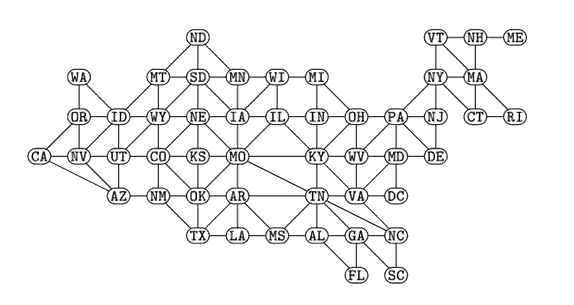
\includegraphics[scale = 0.26]{contiguous-usa-graph}
            %\caption{\tiny{Brain Network}}
            \label{fig:tree}
        \end{minipage}\hfill
        \begin{minipage}[t]{0.48\textwidth}
            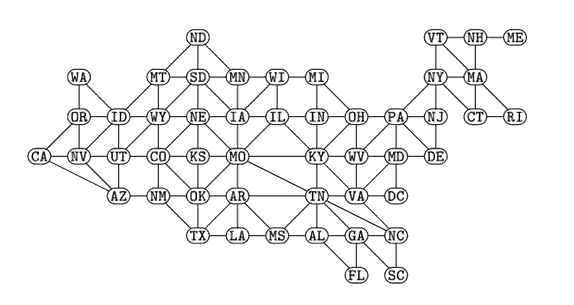
\includegraphics[scale = 0.26]{contiguous-usa-graph}
            %\caption{\tiny{Retweet Network}}
            \label{fig:rand_forest}
        \end{minipage}\hfill
    \end{figure}
    
\begin{itemize}
    \item[-]<1> \tiny Retrieved from:\\ 
    \url{http://networkrepository.com/bn-mouse-visual-cortex-2.php\%} \\ \vspace{-\baselineskip}
    \url{http://networkrepository.com/rt-retweet.php\%}
\end{itemize}

\pause \footnotesize{\hspace{1cm}Brain Network \hspace{3cm} Retweet Network}\\
\pause \footnotesize Mislabeled 100\% of the time

%    bn-mouse-visual-cortex-2\\
%    \begin{itemize}
%        \item Mislabeled as Retweet Network 100\% of the time\\
%    \end{itemize}
%    \centering
%    \includegraphics[scale=0.35]{brain_mouse_graph}\\
%    \tiny Retrieved from: %\url{http://networkrepository.com/bn-mouse-visual-cortex-2.php%}
\end{frame}



\begin{frame}{Miscellaneous Networks}
    contiguous-usa\\
    \begin{itemize}
    \item Collection Hypothesis: Infrastructure Network
    \item Labeled as Cheminformatics Network 100\% of the times\\
    \end{itemize}
    \centering
    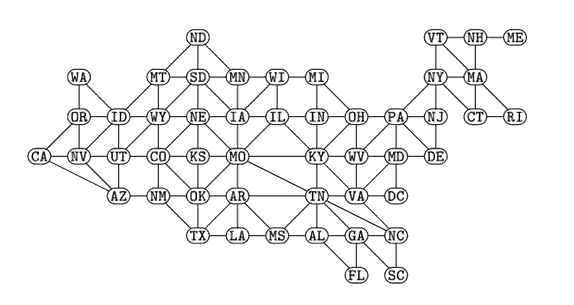
\includegraphics[scale=0.5]{contiguous-usa-graph}
    
    \tiny Retrieved from:  \url{http://mathworld.wolfram.com/images/gifs/ContiguousUSAGraph.gif}
    
\end{frame}


\section{Conclusions}
\frame{\centering \huge Extensions of this Work}


\begin{frame}{Extensions of this Work}

\begin{itemize}
    \item Within Network Science
    \begin{itemize}
        \item Collect more graphs to include more collections in models%Run our algorithms using more graphs
        \item Investigate potential similarities between graph collections (social and web)
        \item Explore new collections, for example, Lexical Networks
    \end{itemize}

    \item Connecting to Graph Theory
    \begin{itemize}
        \item Investigate more comprehensive (random) graph generation models, motivated by similarities discovered
        \item Understand how distinctive, identifying features impact dynamics and behavior on graphs
    \end{itemize}
    
\end{itemize}

\end{frame}


%final thank you slide
\begin{frame}

\begin{center}
{\Huge Thank You!} \\ %\hspace{.2cm}
\begin{figure}
        %\centering
        \begin{minipage}[t]{0.48\textwidth}
        \centering
            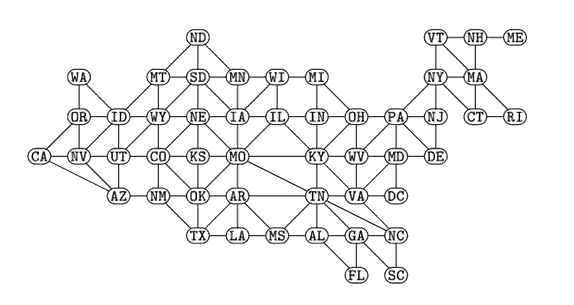
\includegraphics[scale = 0.22]{contiguous-usa-graph}\\
            \scriptsize Supported by NSF Grant DMS-1559912
            %\caption{\tiny{Brain Network}}
            \label{fig:nsf}
        \end{minipage}\hfill
        \begin{minipage}[t]{0.48\textwidth}
        \centering
            
\includegraphics[scale = 0.25]{Valpo}
            %\caption{\tiny{Retweet Network}}
            \label{fig:valpo}
        \end{minipage}\hfill
    \end{figure}


\end{center}

\end{frame}


\begin{frame}{References}
    \begin{itemize}
    \scriptsize{
        \item G. Li, M. Semerci, B. Yener, and M. J. Zaki, Graph classification via topological and label attributes, In 9th Workshop on Mining and Learning with Graphs (with SIGKDD), 2011.
        \item Bonner, Stephen, et al. "Efficient Comparison of Massive Graphs Through The Use Of Graph Fingerprints." Twelfth Workshop on Mining and Learning with Graphs (MLG) Workshop at KDD’16. 2016.
        \item Soundarajan, Sucheta, Tina Eliassi-Rad, and Brian Gallagher. "A guide to selecting a network similarity method." Proceedings of the 2014 SIAM International Conference on Data Mining. Society for Industrial and Applied Mathematics, 2014.
        \item Ryan A. Rossi, Nesreen K. Ahmed, and Others. "An Interactive Network Data Repository." Network Repository. N.p., n.d. Web. 2015.
        \item Maaten, Laurens van der, and Geoffrey Hinton. "Visualizing data using t-SNE." Journal of Machine Learning Research 9.Nov (2008): 2579-2605.
        \item Schutt, Rachel and Cathy O'Neil. Doing Data Science. [Electronic Resource]. Beijing ; Sebastopol : O'Reilly Media, 2013. %EBSCOhost, libdata.lib.ua.edu/login?url= url{http://search.ebscohost.com/login.aspx?direct=true&db=cat00456a&AN=ua.4148576&site=eds-live&scope=site.
        }
    \end{itemize}
\end{frame}


\end{document}